\documentclass[bsc,logo,twoside]{infthesis}

\usepackage{graphicx}
\usepackage{float}
\usepackage{courier}

\title{Prophasis - An IT Infrastructure Monitoring Solution}
\author{Cameron Gray}
\abstract{Prophasis is an IT infrastructure monitoring system that is designed
to suit small to medium size businesses where a system needs to be intuitive to
manage. Management of the entire system can therefore be handled from a single,
responsive web interface. It is also suitable as a one-stop tool with support
for both time series monitoring in addition to real time alerting.
Traditionally two different tools would be needed to gain this level of
monitoring.}

\begin{document}
\maketitle
\tableofcontents

\chapter{Introduction}
\section{Background}
\paragraph*{}
	% TODO: Reword this?
	In recent years, almost all businesses have been expanding their IT
	infrastructure to handle the modern demand for IT systems.  As these systems
	grow and become increasingly important for business operation it is crucial
	that they are sufficiently monitored to prevent faults and periods of downtime
	going unnoticed.  There is already a large market of tools for monitoring IT
	systems however they are designed for use on massive scale networks managed by
	teams of specialised systems administrators.  They are therefore complicated to
	set up and manage and multiple tools are often required to gain a suitable
	level of monitoring.

\paragraph*{}
	For example, tools generally either fall into the category of real time
	alerting (i.e. telling someone when something breaks) and time series
	monitoring (i.e. capturing data about the performance of systems and presenting
	graphs and statistics based on it), there is a large gap in the market for
	tools that provide both of these in one package. This reduces the time required
	to manage the system as it eliminates the need to set up and configure two
	completely separate tools.

\paragraph*{}
	These tools are also generally managed and configured through various
	configuration files split across different machines on the network. This means
	that in order to efficiently use these tools a configuration management system
	such as	Puppet must be used. In a small business with limited IT resources, a
	completely self contained system is often preferable.

\section{Current Landscape}
\paragraph*{}
This section will review current IT infrastructure monitoring systems and
evaluate them on several points as follows:
\begin{itemize}
	\item Support for timeseries monitoring and real time alerting
	\item How they can be configured to monitor custom metrics
	\item How are alert thresholds defined
	\item How configuration and custom code is delivered to nodes (if required)
	\item How the user configures the system
	\item How dependencies are handled
\end{itemize}

\subsection{Nagios}
\paragraph*{Timeseries monitoring and real time alerting}
Nagios is primarily focused at real time alerting and therefore has very little
in the way of timeseries monitoring.  Additional plugins are available which can
be used to graph metrics over time but these cannot be used to make decisions on
the status of a given system or service. All that is supported in terms of
alerting on historical data is to refrain from alerting until a given condition
has been observed in the previous $n$ checks, there is no support for alerting
based on trends in historical data.  Supports basic display of changes in state
of hosts/services over time but not individual metrics.

\paragraph*{Support for custom metrics}
Nagios has support for custom metrics through the NRPE (Nagios Remote Plugin
Executor) plugin. These plugins can be any sort of executable which prints out a
message to represent the data read as well as a specific exit code which defines
the status, for example "OK", "Critical" .etc

\paragraph*{Alert threshold definition}
Thresholds for NRPE agents must be set on the remote server itself.  These
thresholds are passed into the remote plugin as an argument when it is executed
and are used internally by the script to output the appropriate alert level.

\paragraph*{Code/Config delivery to nodes}
Nagios does not have any in built functionality to distribute configuration
files or plugin code to remote nodes. In order to automate this, additional
software such as Puppet would be required.

\paragraph*{How the user configures the system}
Configuration for Nagios is primarily managed through text files stored on disk.
Third party configuration tools are available to allow the system to be
configured through a web interface. Configuration lives on both the Nagios
server as well as on the machines being monitored.

\paragraph*{How dependencies are handled}
Rigid tree - No way to define that a service/host is dependent on a given host
OR another host being available.  This reduces its usefulness in modern networks
where redundancy and failover is commonplace. These are defined in config files
that live on the Nagios server.

\subsection{Icinga 2}
\paragraph*{Timeseries monitoring and real time alerting}
Like Nagios, Icinga's primary focus is around real time alerting however it has
now introduced support for graphing performance metrics.  No support for alerting
based on trends in historical data beyond Nagios's idea of a state change
changing to HARD once it has been observed $n$ times.

\paragraph*{Support for Custom Metrics}
Custom metrics can be written as scripts in any language as long as they echo a
message to describe the status of what they are checkign and use a certain exit
code to define the status e.g. "OK", "CRITICAL", "WARNING".etc.

\paragraph*{Alert threshold definition}
Thresholds are passed into the check commands as command line arguments.
Therefore they are defined on the machines being monitored individually.

\paragraph*{Code/Config delivery to nodes}
Icinga 2 does not have any built-in mechanism to distribute code and config
files to remote hosts. In order for this to be achieved, additional software
such as Puppet would be required.

\paragraph*{How the user configures the system}
Configuration is managed through configuration files stored on disk.
Configuration files exist both on the Icinga server as well as the nodes being
monitored.

\paragraph*{How dependencies are handled}
Same as Nagios with a rigid tree.  No way to define a host/service as being
dependent on one of several different machines as is common in modern
environments with redundancy/failover systems.

\subsection{Munin}
\paragraph*{Timeseries monitoring and real time alerting}
Munin is targeted primarily as a timeseries monitoring tool.  It therefore has
good functionality for graphing data over time.  However, it does not have much
power in the way of alerting other than some very basic functionality where
plugins must manually send out emails/syslog alerts.  This is not really
sufficient for any sort of production use and it instead recommended to use a
tool such as Nagios and push the data from Munin into it.

\paragraph*{Support for custom metrics}
Munin has a simple interface for custom plugins where a plugin is a simple
script that prints out the name and value of the data being collected.  This is
then served by the Munin node which the Munin server contacts over the network
to fetch values from the nodes.

\paragraph*{Alert threshold definition}
Nothing built in, plugins however can create thresholds internally and use them
for alerting (as detailed above) although this isn't really the intended use of
Munin.

\paragraph*{Code/Config delivery to nodes}
Nothing built in, code and config must be distributed manually or automatically
through the use of additional software such as Puppet.

\paragraph*{How the user configures the system}
Configuration is handled through text files stored on disk.  These are stored on
both the Munin server as well as machines being monitored.

\paragraph*{How dependencies are handled}
No dependency functionality.

\section{Improvements}
% TODO: Find a better place for this?
\paragraph*{}
	Prophasis is designed for use in a small to medium business with limited IT
	resources.  They may have a small IT team with limited resources or may not
	even have a dedicated IT team at all, instead relying on one or two employees
	in other roles who manage the business's IT systems on the side of their
	regular jobs. Therefore the system needs to be quick to deploy and manage with
	a shallow learning curve. In order to use the system efficiently there should
	be no requirement for additional tooling to be deployed across the company.

\subsection{Configuration Management}
\paragraph*{}
	It should be possible to manage the configuration of the system from a single
	location.  Prophasis therefore provides a responsive web interface where every
	aspect of the system's operation can be configured, Prophasis then handles
	distributing this configuration to all other machines in the system in the
	background. Custom code for plugins is handled in the same way; it is uploaded
	to the single management machine and is then automatically distributed to the
	appropriate remote machines when it is required.

\subsection{Time Series Monitoring \& Real Time Alerting}
\paragraph*{}
	Prophasis provides both the ability to alert administrators in real time when a
	fault is discovered with the system alongside functionality to collect
	performance metrics over time and use this data to generate statistics about
	how the system has been performing.  This time series data can be used to both
	investigate the cause of a failure in post-mortem investigations in addition to
	being able to be used to predict future failures by looking at trends in the
	collected data.

\subsection{Expandability}
\paragraph*{}
	It is important that a monitoring tool can be expanded to support the
	monitoring of custom hardware and software.  An example of this would be
	hardware RAID cards.  Getting the drive health from these types of devices can
	range from probing for SMART data all the way to communicating with the card
	over a serial port.  It is therefore crucial that Prophasis can be easily
	expanded to support custom functionality such as this. Therefore Prophasis
	supports a system of custom "plugins" which can be written and uploaded to the
	monitoring server where they can then be configured to monitor machines. These
	plugins are designed to be self contained and to follow a well defined and
	documented structure.  This provides scope for a plugin "marketplace" therefore
	eliminating the need for every user to implement custom monitoring code for the
	systems they are using.


\chapter{Design}
\section{Technology Choice}
\subsection{Why Python?}
\subsection{Why HTTPS?}

\section{System Structure}
\paragraph*{}
	The system is split up into three separate components; Web, Core and Agent. Web
	and core both share the same relational database allowing data to be shared
	between them.  Figure \ref{system_structure} shows the individual components of
	the system and how they all interact.

\begin{figure}[H]
	\caption{Diagram showing the layout of the components of the system}
	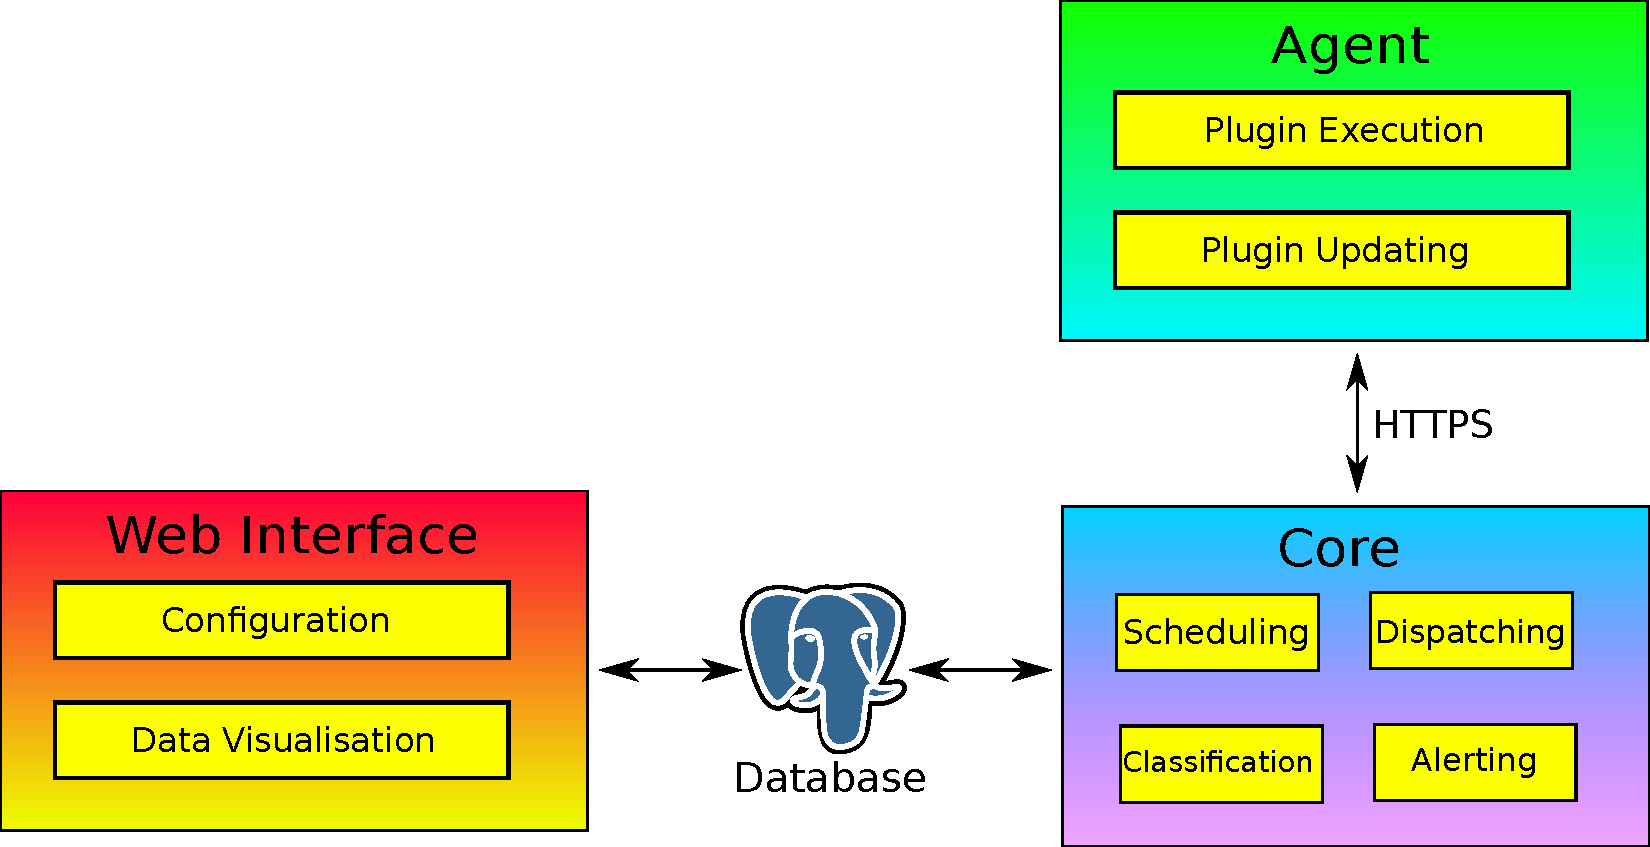
\includegraphics[scale=0.5]{assets/system_structure.pdf}
	\label{system_structure}
\end{figure}

\subsection{Agent}
\paragraph*{}
	The agent runs on every machine that is being monitored and provides an API for
	communication with the monitoring server.  It listens on port 4048 (by default)
	and exposes an HTTPS API.  This API includes methods to check the version of a
	plugin currently installed on the agent, a method to push updated plugins to
	the agent and another method to execute a plugin and to retrieve the value and
	message produced by it.

\paragraph*{}
	The agent's API is authenticated using a long, pre-shared key of which a salted
	hash is stored on the agent in a configuration file.  Being hashed prevents
	users who may have access to read the configuration file (possibly through
	misconfiguration) from getting the key to be able to communicate with the
	agent.

\subsection{Core}
\paragraph*{}
	The core runs on the machine that is performing the monitoring, it has several
	different roles; scheduling, dispatching, classification and alerting.

\subsubsection{Scheduling}
\paragraph*{}
	The core is responsible for looking at the schedules stored in the database and
	executing the appropriate checks on the correct hosts at the correct time.
	There is a configuration value for "maximum lateness" that defines how late
	after its defined time slot a check can be executed.  The core repeatedly
	checks the database looking at the intervals for each schedule along with the
	time at which a given schedule was last executed.  If it decides that a
	schedule is due to be executed it passes this onto the dispatcher.

\paragraph*{}
	Figure \ref{scheduler_flowchart} describes how the scheduler operates.  Each
	schedule has a \linebreak\texttt{start\_timestamp} which is defined by the user
	when the schedule is created, an \texttt{interval} which is how often the
	schedule executes and a value for \texttt{execute\_next} which is the timestamp
	that the schedule is next to be executed.  When the scheduler starts up it
	first gets all schedules that do not have an \texttt{execute\_next} value -
	These are schedules that have never run.  It then calls
	\texttt{walk\_execute\_next} which is a simple algorithm that "fast forwards"
	the \texttt{execute\_next} value until it reaches a timestamp that is in the
	future.  It then retrieves any schedules that are due to be executed
	(\texttt{execute\_next} is in the past) and executes them, it then calls
	\texttt{walk\_execute\_next} on each of these to set the \texttt{execute\_next}
	value to the time that the schedule should be run again.  The algorithm will
	then wait for 1 second before executing the process again.

\begin{figure}[H]
	\caption{Flowchart describing the operation of the scheduler}
	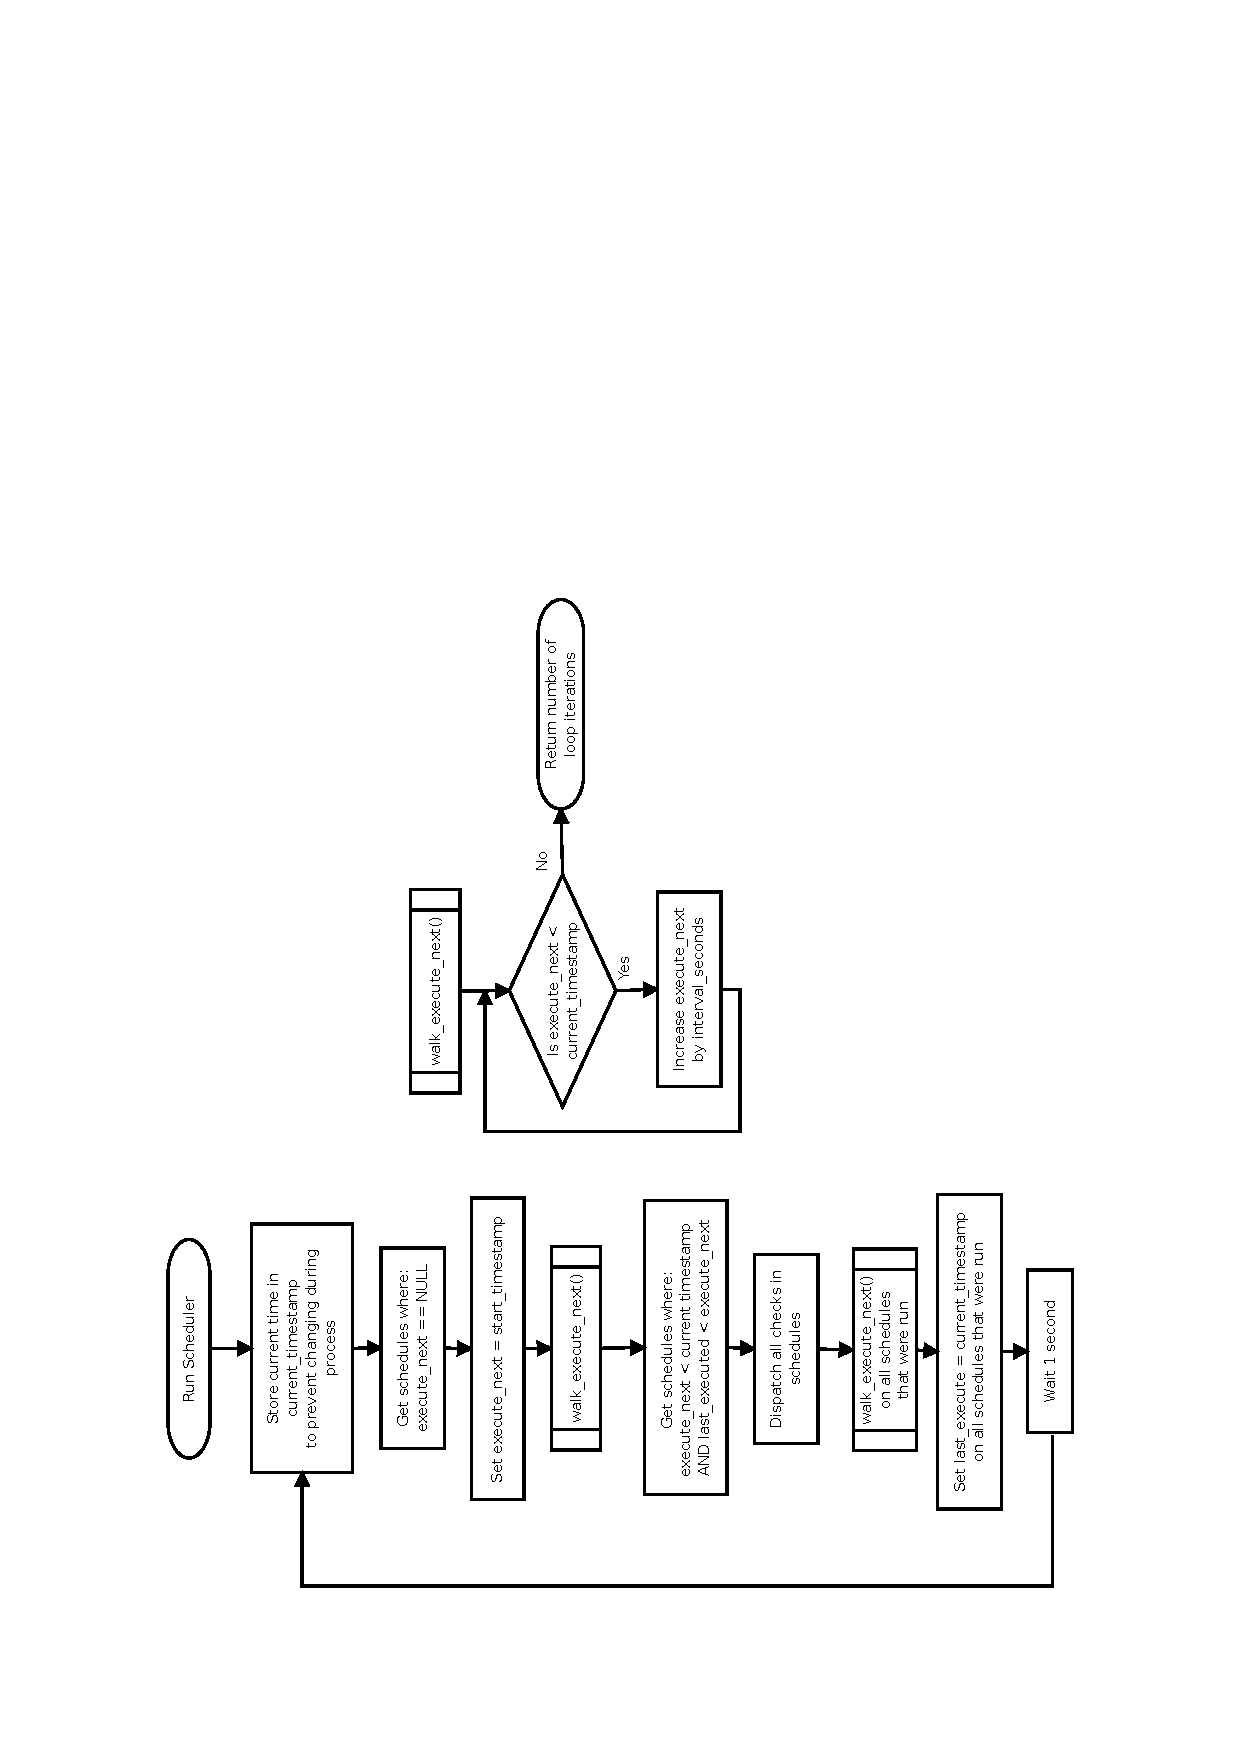
\includegraphics[scale=0.7, angle=-90]{assets/scheduler_flowchart.pdf}
	\label{scheduler_flowchart}
\end{figure}


\subsubsection{Dispatching}
\paragraph*{}
	The dispatcher component of the core is responsible for issuing checks to
	agents when they are due to be run (as decided by the scheduler).  Checks may
	take some time to execute so executing these all in series would all be
	impractical. The solution for this was for the dispatcher to spawn a process
	for each agent that it is currently executing checks for.  Each process
	maintains a queue of plugins that are due to be executed and issues them to the
	agent in the order that they were dispatched.  This way only one plugin can be
	executing on a given agent at any moment in time.  This both prevents agents
	from becoming overwhelmed and means that plugin developers do not need to be
	concerned about other plugins interfering with their plugin.  Figure
	\ref{dispatcher_flowchart} shows the operation of the dispatcher.

\begin{figure}[H]
	\caption{Flowchart describing the operation of the dispatcher}
	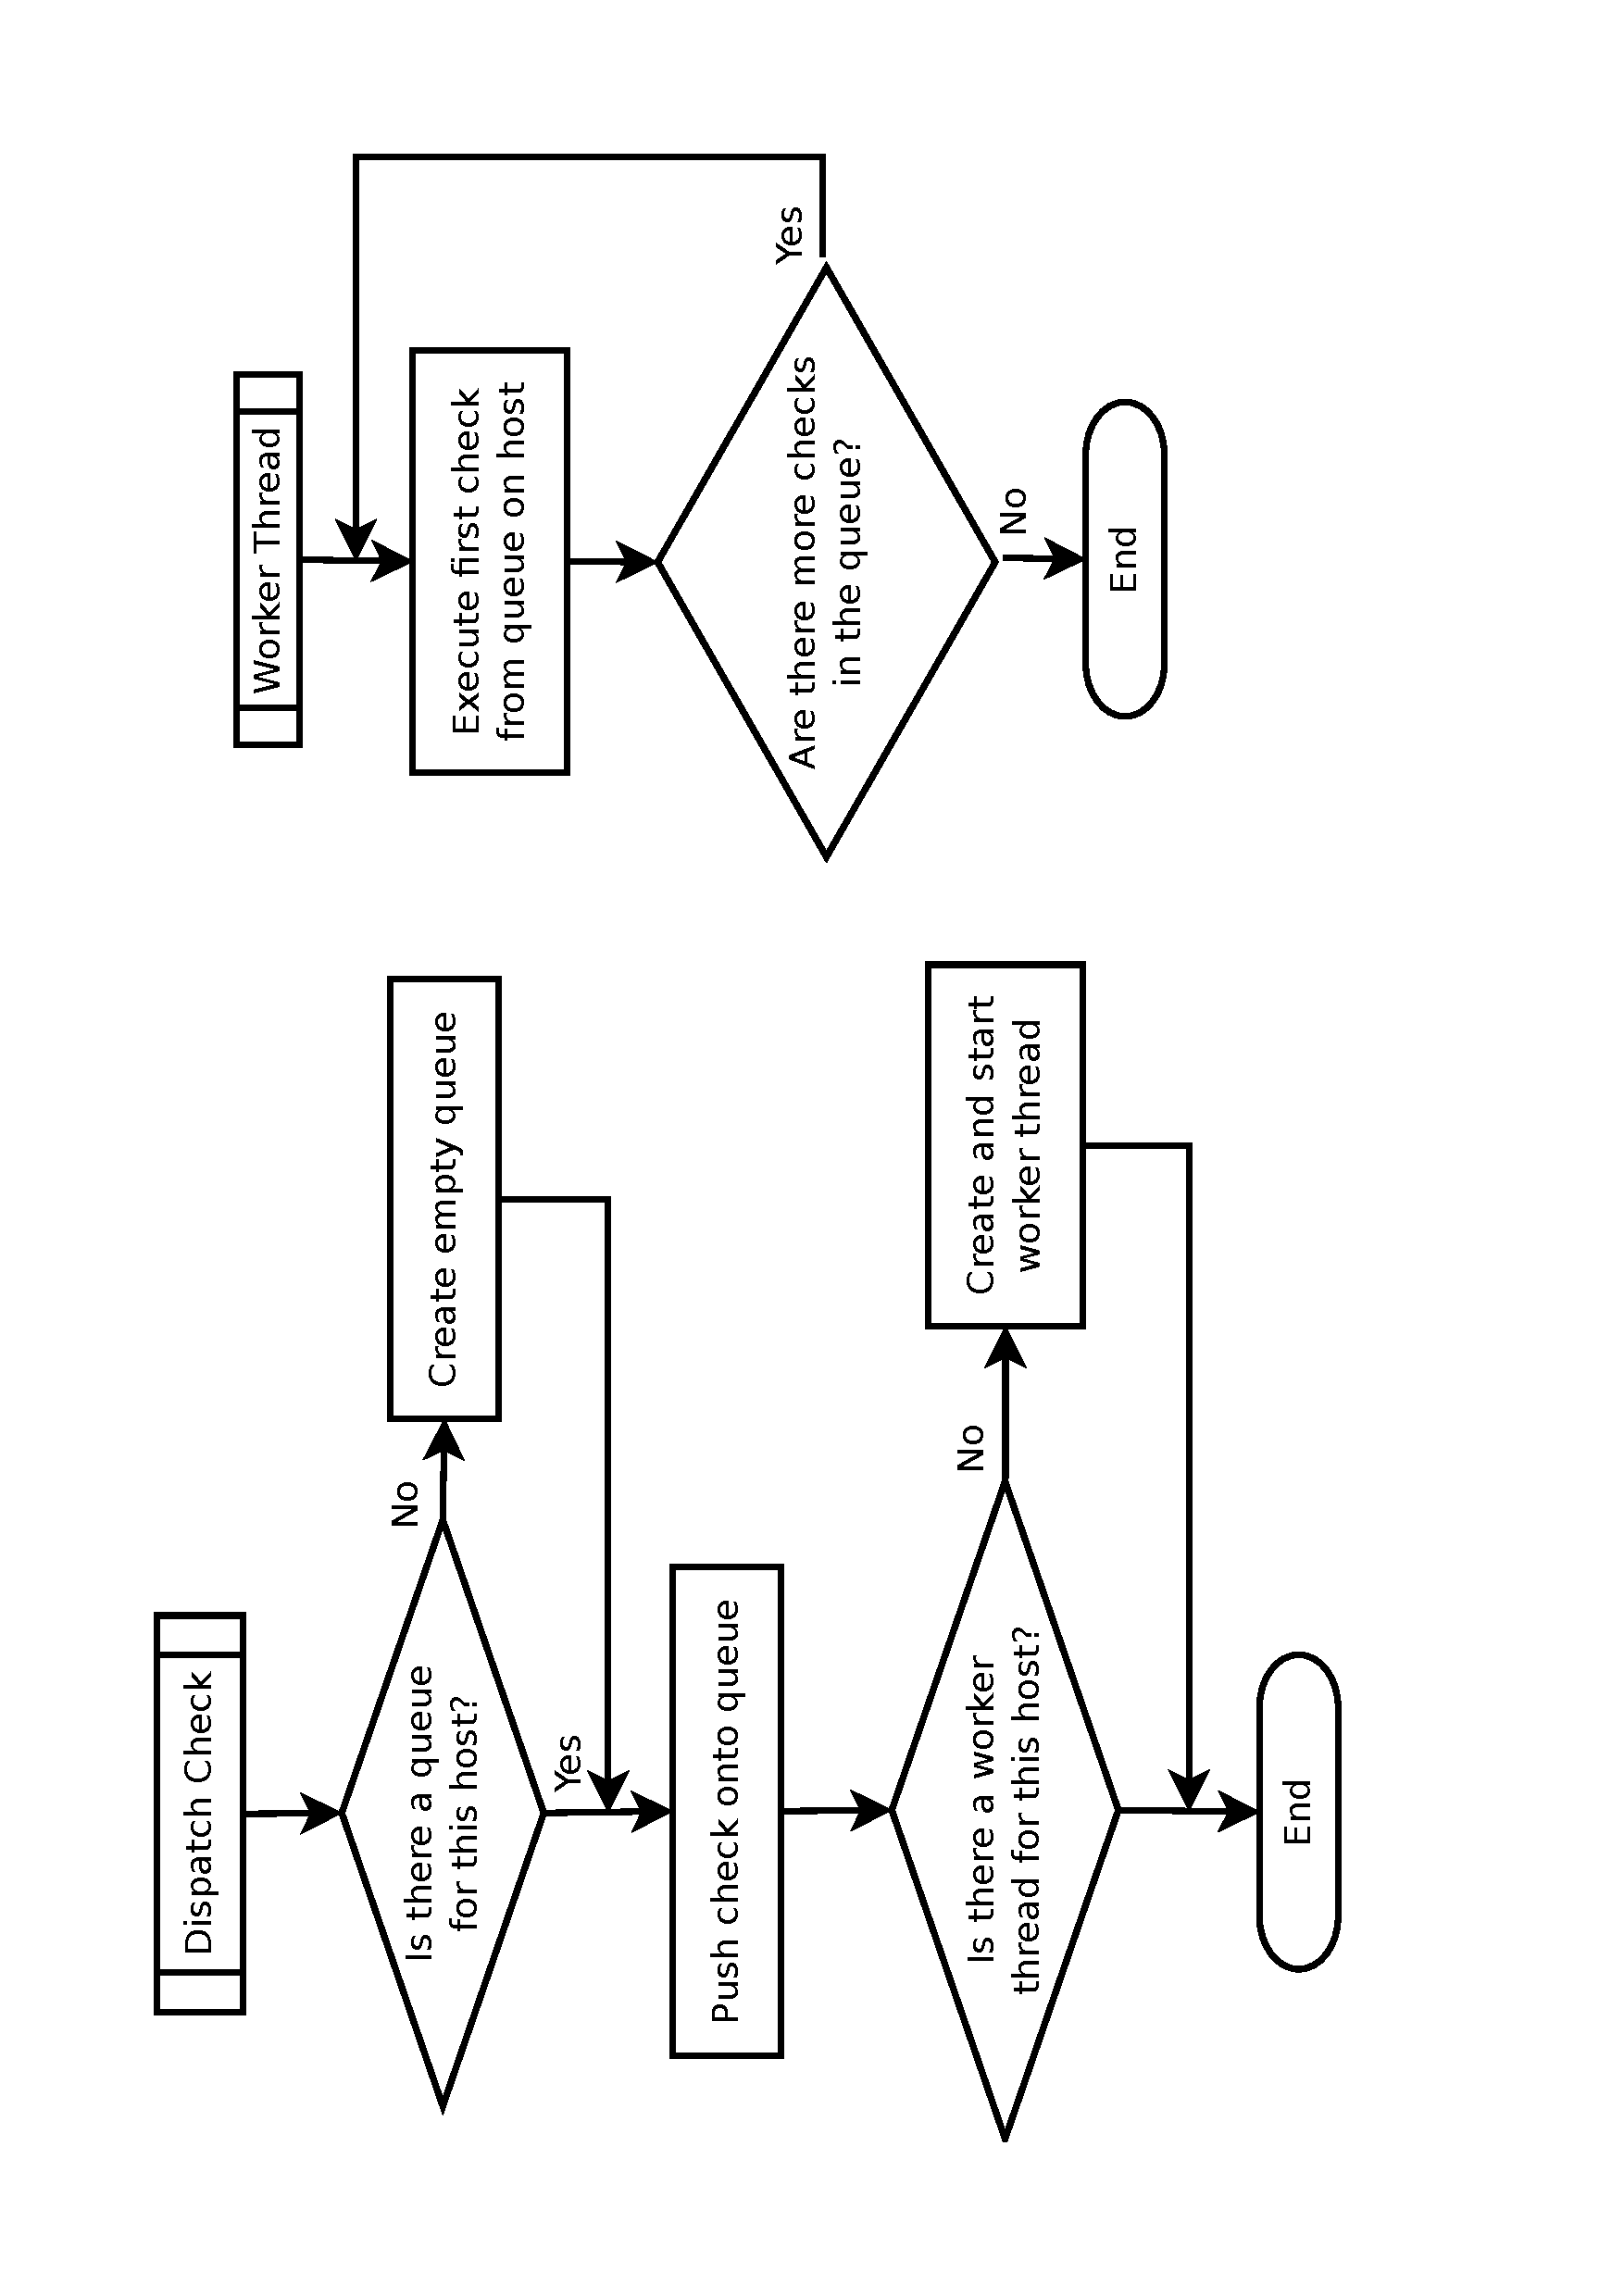
\includegraphics[scale=0.8, angle=-90]{assets/dispatcher_flowchart.pdf}
	\label{dispatcher_flowchart}
\end{figure}

\paragraph*{Communication Between Core and Agent}
	When a check is dispatched, the core and agent communicate to first of all
	establish if the agent already has the correct version of the plugin due to be
	executed installed. If it does not then an update will be sent to the agent.
	Once this is done the core will then request the agent to execute the plugin
	and the data will be returned for classification.  Figure
	\ref{core_agent_communication} describes the communication between the core and
	the agent.

\begin{figure}[H]
	\caption{Flowchart describing the communication between the core and the agent
		when a check is dispatched}
	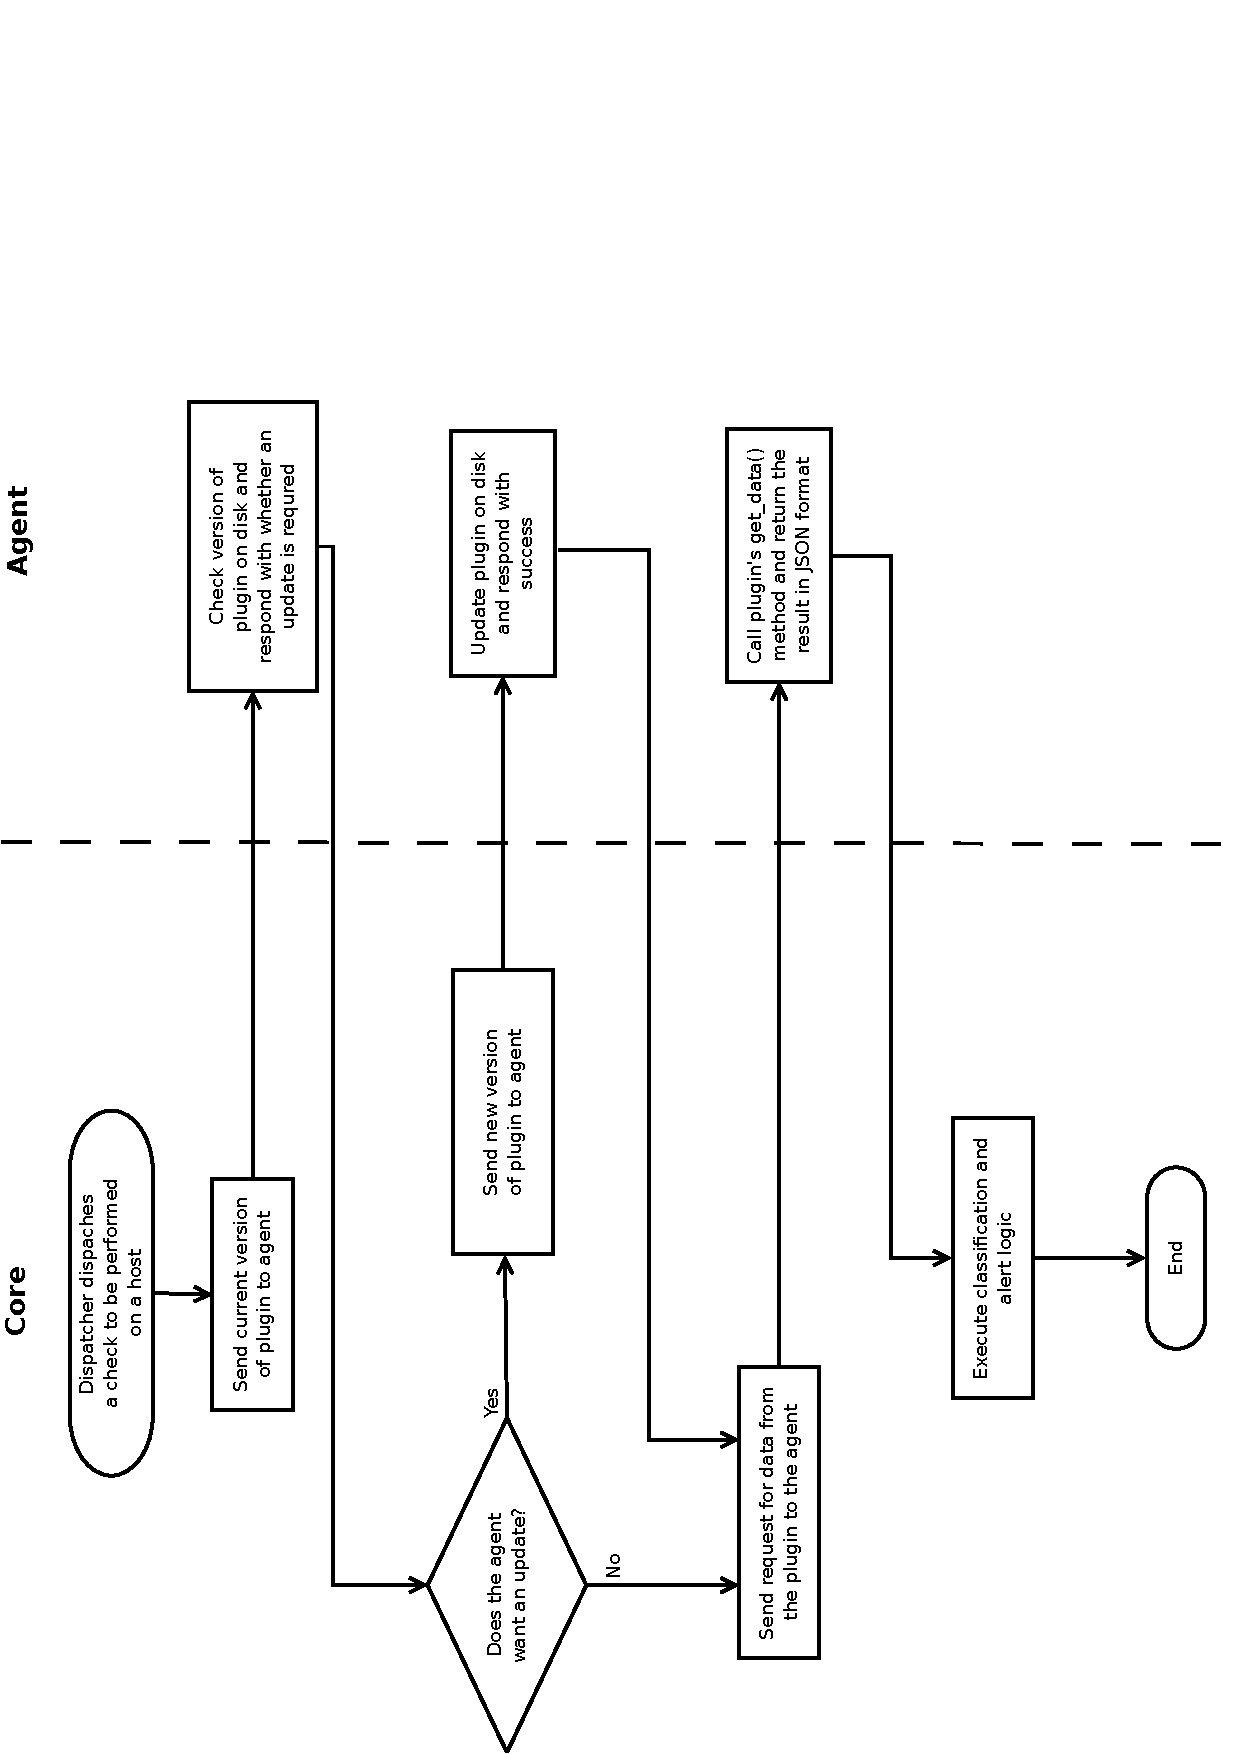
\includegraphics[scale=0.6, angle=-90]{assets/core_agent_communication.pdf}
	\label{core_agent_communication}
\end{figure}

\subsubsection{Classification}
\paragraph*{}
	When data is collected from an agent, it needs to be classified as "ok",
	"major", "minor", "critical" or "unknown".  Classification is performed by lua
	code that is stored alongside each plugin.  When the core finishes collecting a
	from an agent it will retrieve the classification code for the plugin and
	execute it in a sandboxed lua runtime environment.  The result of the
	classification is then stored in the database.  The use of Lua code provides
	total flexibility, classifications can be as simple as comparing values to a
	threshold or could go as far as looking at previous historical values and
	classifying based on a trend in the data. Plugins define how many previous
	historical values they want to classify on ($n$), the plugin's classifier code
	is then executed with two Lua tables, one containing the previous $n$ "values"
	stored and the other containing the previous $n$ "messages".

\subsubsection{Alerting}
\paragraph*{}
	Once the core has classified a piece of data, the core now needs to work out
	whether it needs to send an alert or not.  To do this it looks at the previous
	state for the plugin and host along with the current state.  It then looks
	through the database for alerts that match that state transition and are
	applicable to the host/plugin combination.  If any alerts match it will call
	the alert module to send the alert out to inform the necessary people about the
	state change.

\subsection{Web Interface}
\paragraph*{}
	Prophasis provides a web interface for both configuring the system and viewing
	collected data.  The interface is designed to be clear and easy to understand
	for users.  It is also built to be fully responsive so will work correctly on
	mobile device without any loss of functionality.  Designing it to be responsive
	was the aim from the outset as servers often fail when the administrator may
	not currently be in easy reach of a computer so will need to use a mobile
	device to investigate the issue.

\paragraph*{}
	The web interface will connect to the same database as the core, the web
	interface will update the configuration data stored in this database and will
	retrieve the data about hosts.

\paragraph*{}
	The web interface provides dashboards for visualisation of data collected from
	plugins.  The collected data can then be displayed using graphs, tables, lists
	of messages or any other way that suits the type of data collected.

\section{Monitoring Methodology}
\subsection{Host Management}
\paragraph*{}
	In Prophasis, a "host" refers to a single machine that is being monitored. To
	aid management and organisation, it is possible to organise hosts into "Host
	Groups."  These can be comprised of hosts or other groups and can be used in
	place of hosts when defining services and checks.  Hosts can be grouped in
	various ways such as their role (Webserver, VM Host), hardware configuration
	(Hardware RAID, Contains GPU), location (Edinburgh Office, Datacenter) or any
	other way that makes sense given the specific implementation.

\subsection{Plugins}
\paragraph*{}
	A "plugin" is a package that checks a single attribute of a system.  For
	example a plugin could check the CPU load of a given machine or be used to
	check the health of all the hard drives in a system.  Plugins are implemented
	as Python modules that implement a specific API, they can return both a "value"
	(a numerical representation of the data they collected) and/or a "message" (a
	string representation of the collected data).  Plugins are then packaged in a
	.tar.gz archive along with a manifest JSON file which contains information
	about the plugin for use when it is installed.

\paragraph*{}
	Plugins are automatically distributed from the core to remote machines and when
	executed by the agent the value and message are returned to the core for
	classification and storage in the database.

\subsection{Checks}
\paragraph*{}
	A "check" is a named set of hosts/host groups and a set of plugins to be
	executed on them.  When a check is executed, all of the plugins specified in
	the check will be executed across all of the hosts specified in the check.

\paragraph*{}
	Checks allow logical grouping of various plugins.  For example you may have a
	check for "Webserver Resource Usage" which will execute plugins to check the
	CPU load and memory across all hosts in the "Webservers" host group.

\subsection{Schedules}
\paragraph*{}
	A schedule defines when one or more checks are to be executed.  Each schedule
	can contain multiple "intervals" which define when the check is run.  An
	interval has a start date/time and a time delta that defines how regularly it
	is to be implemented.

\subsection{Services}
\paragraph*{}
	Services can be used to define a more fine grained representation of how the
	availability of a host affects the performance of the system overall.  A
	service is defined in terms of "dependencies" and "redundancy groups". Each
	dependency represents a host that must be operational for the service to work.
	A redundancy group can contain multiple hosts where at least one must be
	operational for the service to work.

\paragraph*{}
	As an example, you may have a "Website" service that has a dependency on the
	single router but has a redundancy group containing multiple webservers.
	Therefore, if the router fails then the website will be marked as failed
	however if one of the webservers fails but at least one other webserver is
	still operational, the website service will only be marked as degraded.

\paragraph*{}
	The use of services provides a clearer view of the impact of a given failure on
	the functionality of the network.  It also allows alerts to be set up so that
	they are only triggered when the service functionality is severely impacted and
	prevents alerts from being sent out for host failures that do not have a severe
	impact.

\subsection{Alerts}
\paragraph*{}
	In Prophasis, alerts are set up to communicate with a specific person/group of
	people in a certain situation.  Alerts are defined in terms of to/from stage
	changes where an alert will be sent if the state of a host/service changes from
	one state to another (e.g. "ok" to "critical").  These can then be restricted
	to certain hosts, host groups, services, plugins and checks.

\paragraph*{}
	The system supports "alert modules" - Python modules that are used to send
	alerts using various methods.  Examples of alert modules could be email, SMS or
	telephone call.

\paragraph*{}
	Multiple alerts can be set up to handle different severities of issues.  For
	example, if a redundant service becomes degraded, a SMS or email message may be
	sufficient but if a service becomes critical it may be desirable to use a
	telephone call to gain quicker attention.

\chapter{Implementation}
\section{Technologies}
\paragraph*{}
	The vast majority of the system is implemented in Python 3.  This allows for a
	large variety of modules to be used during development. Python is also widely
	available on UNIX systems and is easy to install on machines where it is not
	included.

\paragraph*{}
	The Python "Virtual Environment" (Virtualenv) system is also extremely useful
	in this system.  It allows all dependencies to be kept totally separate from
	the rest of the system, this is particularly important for the agent as it
	ensures that the agent cannot interfere with the Python environment of the
	systems it is running on.

\subsection{Flask Web Framework}
\paragraph*{}
	The agent and web interface are both built using the Flask web framework which
	handles routing URLs to the correct Python functions as well as handling
	request data and building the correct HTTP responses. The agent purely uses the
	routing and request/response functionality provided by Flask whereas the web
	interface also uses Flask's bundled templating engine, Jinja2, to render the
	HTML pages that are displayed to the user. The web interface also uses the
	Flask-Login package to provide login and user session management functionality.

\subsection{Tornado HTTP Server}
\paragraph*{}
	While Flask does provide a built in webserver, it is only designed for
	development	use.  In order to provide a production suitable web server for the
	%TODO Did we use Tornado for the web interface too?
	agent.  Tornado uses the uWSGI interface provided by Flask.  Tornado was chosen
	as it can easily be integrated directly into the Flask application and
	therefore does not require any sort of external webserver to be
	installed/configured on the system.

\subsection{SQLAlchemy ORM}
\paragraph*{}
	All database functionality in Prophasis is handled through the SQLAlchemy ORM
	which abstracts the database into a set of Python classes (known as models).
	This not only reduces development time, it also reduces the likelihood of
	errors as all of the database queries are generated by the library rather than
	being handwritten.  The SQLAlchemy models file can also be shared between both
	the web interface and the core preventing duplication of database query logic.

\subsection{Lupa}
\paragraph*{}
	Lupa provides an interface between the system's Lua runtime and Python.  It is
	used by Prophasis to execute the user provided Lua code that is used to
	classify the results of checks. A sandboxed Lua environment is configured to
	prevent this user provided code from performing undesired operations.
	Sandboxing is covered further in section \ref{classification_sandboxing}.

\subsection{PostgreSQL Database}
\paragraph*{}
	Prophasis has been officially developed to support PostgreSQL databases,
	however through the use of an ORM it is possible to easily move to different
	database platforms such as MySQL or Oracle.  SQLAlchemy transparently handles
	the difference between different database platforms when generating its
	queries.

\subsection{File path thingy}

\section{Plugin Interface}
\begin{itemize}
	\item Explain structure of a plugin
	\item UML Diagram?
	\item Why Lua for classification logic?
\end{itemize}

\section{Database Design}

\section{Web Interface}
\begin{itemize}
	\item Go into detail about web structure WRT templates, assets.etc
\end{itemize}

\section{Core}
\subsection{Dispatcher}
\paragraph*{}
	The dispatcher is the system which sends off requests to the agent and waits
	for the responses back which are then classified and then stored in the
	database.  Due to the time it may take to execute some checks it would be
	impractical to execute them in series, therefore the dispatcher is
	multi-threaded.

\paragraph*{}
	The Prophasis dispatcher uses Python's built in "multiprocessing" library. This
	provides various methods to manage processes as well as thread-safe data
	structures for communicating between them.  The dispatcher uses
	\texttt{multithreading.Process} to spawn worker processes and uses
	\texttt{multiprocessing.Queue} to define thread safe queues for passing data
	into these worker processes.

\paragraph*{Fork vs Spawn}
	The multiprocessing library supports three different ways to start a process.
	By default on UNIX systems it uses \texttt{os.fork()} to fork the existing
	process. This is unsuitable in this situation as the process creates a copy of
	the already open database connection - this causes conflicts when the workers
	try to write to the database.  The solution to this is to tell the
	multiprocessing library to use the "spawn" context (the default on Windows)
	which will create a fresh Python interpreter process, this prevents open
	handles from being carried over into the child process. Using spawn is
	comparatively slower than forking the process but since we are only creating
	%TODO Better wording than "real world timescale"? worker processes when
	schedules are called (which is on a real world timescale), this difference will
	not be noticeable.

\subsection{Classification}
\paragraph*{}
	When data is collected from the agent it needs to be "classified" to determine
	whether it is "ok", "major", "critical".etc.  Classification is done by Lua
	code that is bundled with the plugin and can also be modified by the user
	through the web interface.  The Lua classification code is stored in the
	database for ease of modification.  The "lupa" Python library is used to
	integrate the Lua runtimes into the Python code.

\subsubsection{Sandboxing}
\label{classification_sandboxing}
\paragraph*{}
	Classification code is executed directly on the machine under the same user as
	the core.  Since this classification code can be changed through the Prophasis
	web interface it is critical that this code cannot perform malicious operations
	on the system.  In order to resolve this, a Lua sandbox is created.  This is
	done by creating a Lua table with only specific, trusted functions such as
	\texttt{math} and \texttt{ipairs} added to it.  Lua's \texttt{setfenv} (set
	function environment) function is then called to ensure that all user provided
	code is executed inside this sandbox and can therefore not access more risky
	operating system functions such as file handling.

\subsubsection{Functions}
\paragraph*{}
	In order to make developing classification code easier, several predefined
	functions are provided to handle common operations such as
	\texttt{arrayMax(array)} which will return the maximum value in an array and
	\texttt{arrayContains(array, value)} which returns a boolean defining whether
	the given value is in the array or not.  These functions are stored in a
	separate Lua file and are included before the user provided classification code
	before it is executed.

\subsubsection{Handling Errors}
\paragraph*{}
	When dealing with user defined code, there is always the potential for errors
	to occur when the classification code is executed.  In this situation the
	system will automatically fall back and classify the result as "unknown". The
	error will also be logged within Prophasis and can be easily viewed by the user
	in the web interface's "System Logs" area.

\begin{itemize}
	\item Scheduling
	\item Multi-threaded dispatcher
\end{itemize}

\section{Agent}
\paragraph*{}
	The agent is implemented using the Flask web framework to expose a HTTPS API
	that the core communicates with.  Requests are sent to the agent using regular
	HTTP GET and POST requests with information passed using URL parameters or HTTP
	form data respectively.  Responses are formatted as JSON.  The Tornado HTTP
	server is used to handle incoming HTTP connections and communicates with Flask
	through using uWSGI.

\paragraph*{Authentication}
	In order to prevent unauthorised actions being performed on the agent, the core
	must authenticate with every request.  The agent stores a hash of a long
	authentication key in its configuration file. This key is generated on agent
	installation and is different for every agent. This ensures that if the key for
	one agent is obtained, an attacker cannot access every other agent on the
	network. Storing a hash means that if someone was able to read the agent
	configuration file they cannot obtain the authentication key which could have
	allowed them to execute code as the agent's user which may have higher
	privileges than their user. HTTP's basic access authentication is used which
	allows a username and password to be easily sent along with an HTTP request, in
	this situation the username is "core" and the password is the authentication
	key.  A Python decorator (\texttt{@requires\_auth}) is applied to functions
	that require authentication which will verify the authentication token and only
	allow the function to execute if the token is correct, otherwise it will
	respond with HTTP error 401 (Unauthorised). Using a decorator dad

\begin{itemize}
	\item Communication
	\item Authentication
\end{itemize}

\chapter{Testing}
\begin{itemize}
	\item Unit testing
	\item Use within Tardis \& Lynchpin
\end{itemize}

\chapter{Evaluation}

\chapter{Conclusion}

\end{document}
